\chapter{Seuil de rentabilité}

Ce chapitre sera consacré à l'étude de problèmes financiers.

\section{Recherche de seuil}

Nous nous intéresserons ici aux entreprises qui produisent un seul article. Pour pouvoir en fabriquer en quantité, elles ont un certain nombre de frais.

Des frais sont liés à l'existence de l'entreprise (local à louer, machines à acheter, etc.) et d'autres à la production (matière première, etc). On appelle les premiers les \emph{frais fixes}\index{seuil de rentabilité!frais fixes}, notés $f_f$ et les second les \emph{frais variables}\index{seuil de rentabilité!frais variables}, notés $f_v$. Bien entendu, les frais fixes ne dépendent pas du nombre d'objets produits, alors que les seconds oui.

Secondement, l'entreprise vend ses produits, ce qui génère un \emph{gain}\index{seuil de rentabilité!gain}, noté $g$. L'ensemble des gains pour la vente de toute la production est ce qu'on appelle en économie le chiffre d'affaire. Dans tout ce chapitre, nous considérerons que l'ensemble de la production est systématiquement vendue.

Le \emph{seuil de rentabilité}\index{seuil de rentabilité} est le nombre d'objet qu'il faut produire afin d'équilibrer les gains et les frais. Il se trouve en résolvant l'équation

$$
f_v \cdot x + f_f = g\cdot x
$$
où $x$ est le nombre de marchandise produite. La fonction $f_v + f_f \cdot x$ représente l'ensemble des frais de l'entreprise pour produire $x$ marchandises, alors que la fonction $g\cdot x$ l'ensemble des gains liés à la vente de $x$ marchandises.

\begin{exemple}\label{ex_seuil}
Mon amie décide de se lancer dans la production de scoubidous. Pour cela, elle doit acheter une tresseuse de scoubidous à $100$ Frs. Elle a calculé que chaque scoubidou lui coûte $0.50$ Frs de fil. Enfin, elle décide de les vendre $3$ Frs pièce. Quel est son seuil de rentabilité ?

En analysant le problème, on trouve :
$$
\left\{
\begin{array}{l}
f_f = 100\\
f_v = 0.5
g = 3
\end{array}
\right.
\Rightarrow
\left\{
\begin{array}{l}
f(x) = 0.5 x + 100\\
g(x) = 3x
\end{array}
\right.
$$
On doit donc résoudre l'équation
$$
\begin{array}{lcl}
0.5 x + 100 &=& 3x \ssi \\
100 &=& 2.5 x \ssi \\
40 &=& x
\end{array}
$$
Son seuil de rentabilité est donc de $40$ pièces, c'est-à-dire que si elle en produit moins elle perd de l'argent, et elle commence à en gagner à $41$ pièces.
\end{exemple}

\subsection{Représentation}

On vient de le voir, la situation peut être explicitée sous la forme de deux fonctions :
$$
\begin{array}{l}
f(x) = f_v \cdot c + f_f \mbox{ (les frais)}\\
g(x) = g\cdot x \mbox{ (les gains)}
\end{array}
$$

Or il s'agit de deux fonctions affines dont nous avons parlé à la section~\ref{fct_affine}. Puisque $x$ ne peut être que positif (il est peu probable de produire un nombre négatif de marchandise) et que les images des nombres positifs par $f$ et $g$ sont aussi positives, nous nous contenterons de représenter la situation dans le premier cadran, c'est-à-dire le quart supérieur droite.

Le seuil de rentabilité est le moment où $f(x) = g(x)$, et donc les deux graphes passent par le point $\left(x;f(x)\right) = \left(x;g(x)\right)$. Ainsi, puisque les deux droites passent par ce point, elles se coupent au seuil de rentabilité.

Pour une représentation un peu précise, il convient de représenter chaque droite en utilisant l'image de $0$ (l'ordonnée à l'origine) et l'image d'un nombre suffisamment grand (en général, deux fois le seuil de rentabilité).

\begin{exemple}
Reprenons l'exemple~\ref{ex_seuil} : nous avons les deux fonctions suivantes :
$$
\left\{
\begin{array}{l}
f(x) = 0.5 x + 100\\
g(x) = 3x
\end{array}
\right.
$$
On sait déjà que le seuil est à $40$ pièces, nous allons donc calculer les images de $0$ et de $80$ :
$$
\left\{
\begin{array}{l}
f(0) = 0.5 \cdot 0 + 100 = 100 \Rightarrow (0;100)\\
g(0) = 3\cdot 0 = 0 \Rightarrow (0;0)
\end{array}
\right.
\mbox{ et }
\left\{
\begin{array}{l}
f(80) = 0.5 \cdot 80 + 100 = 140 \Rightarrow (0;140)\\
g(80) = 3\cdot 80 =240 \Rightarrow (0;240)
\end{array}
\right.
$$
On représente donc la situation ainsi :
\begin{center}
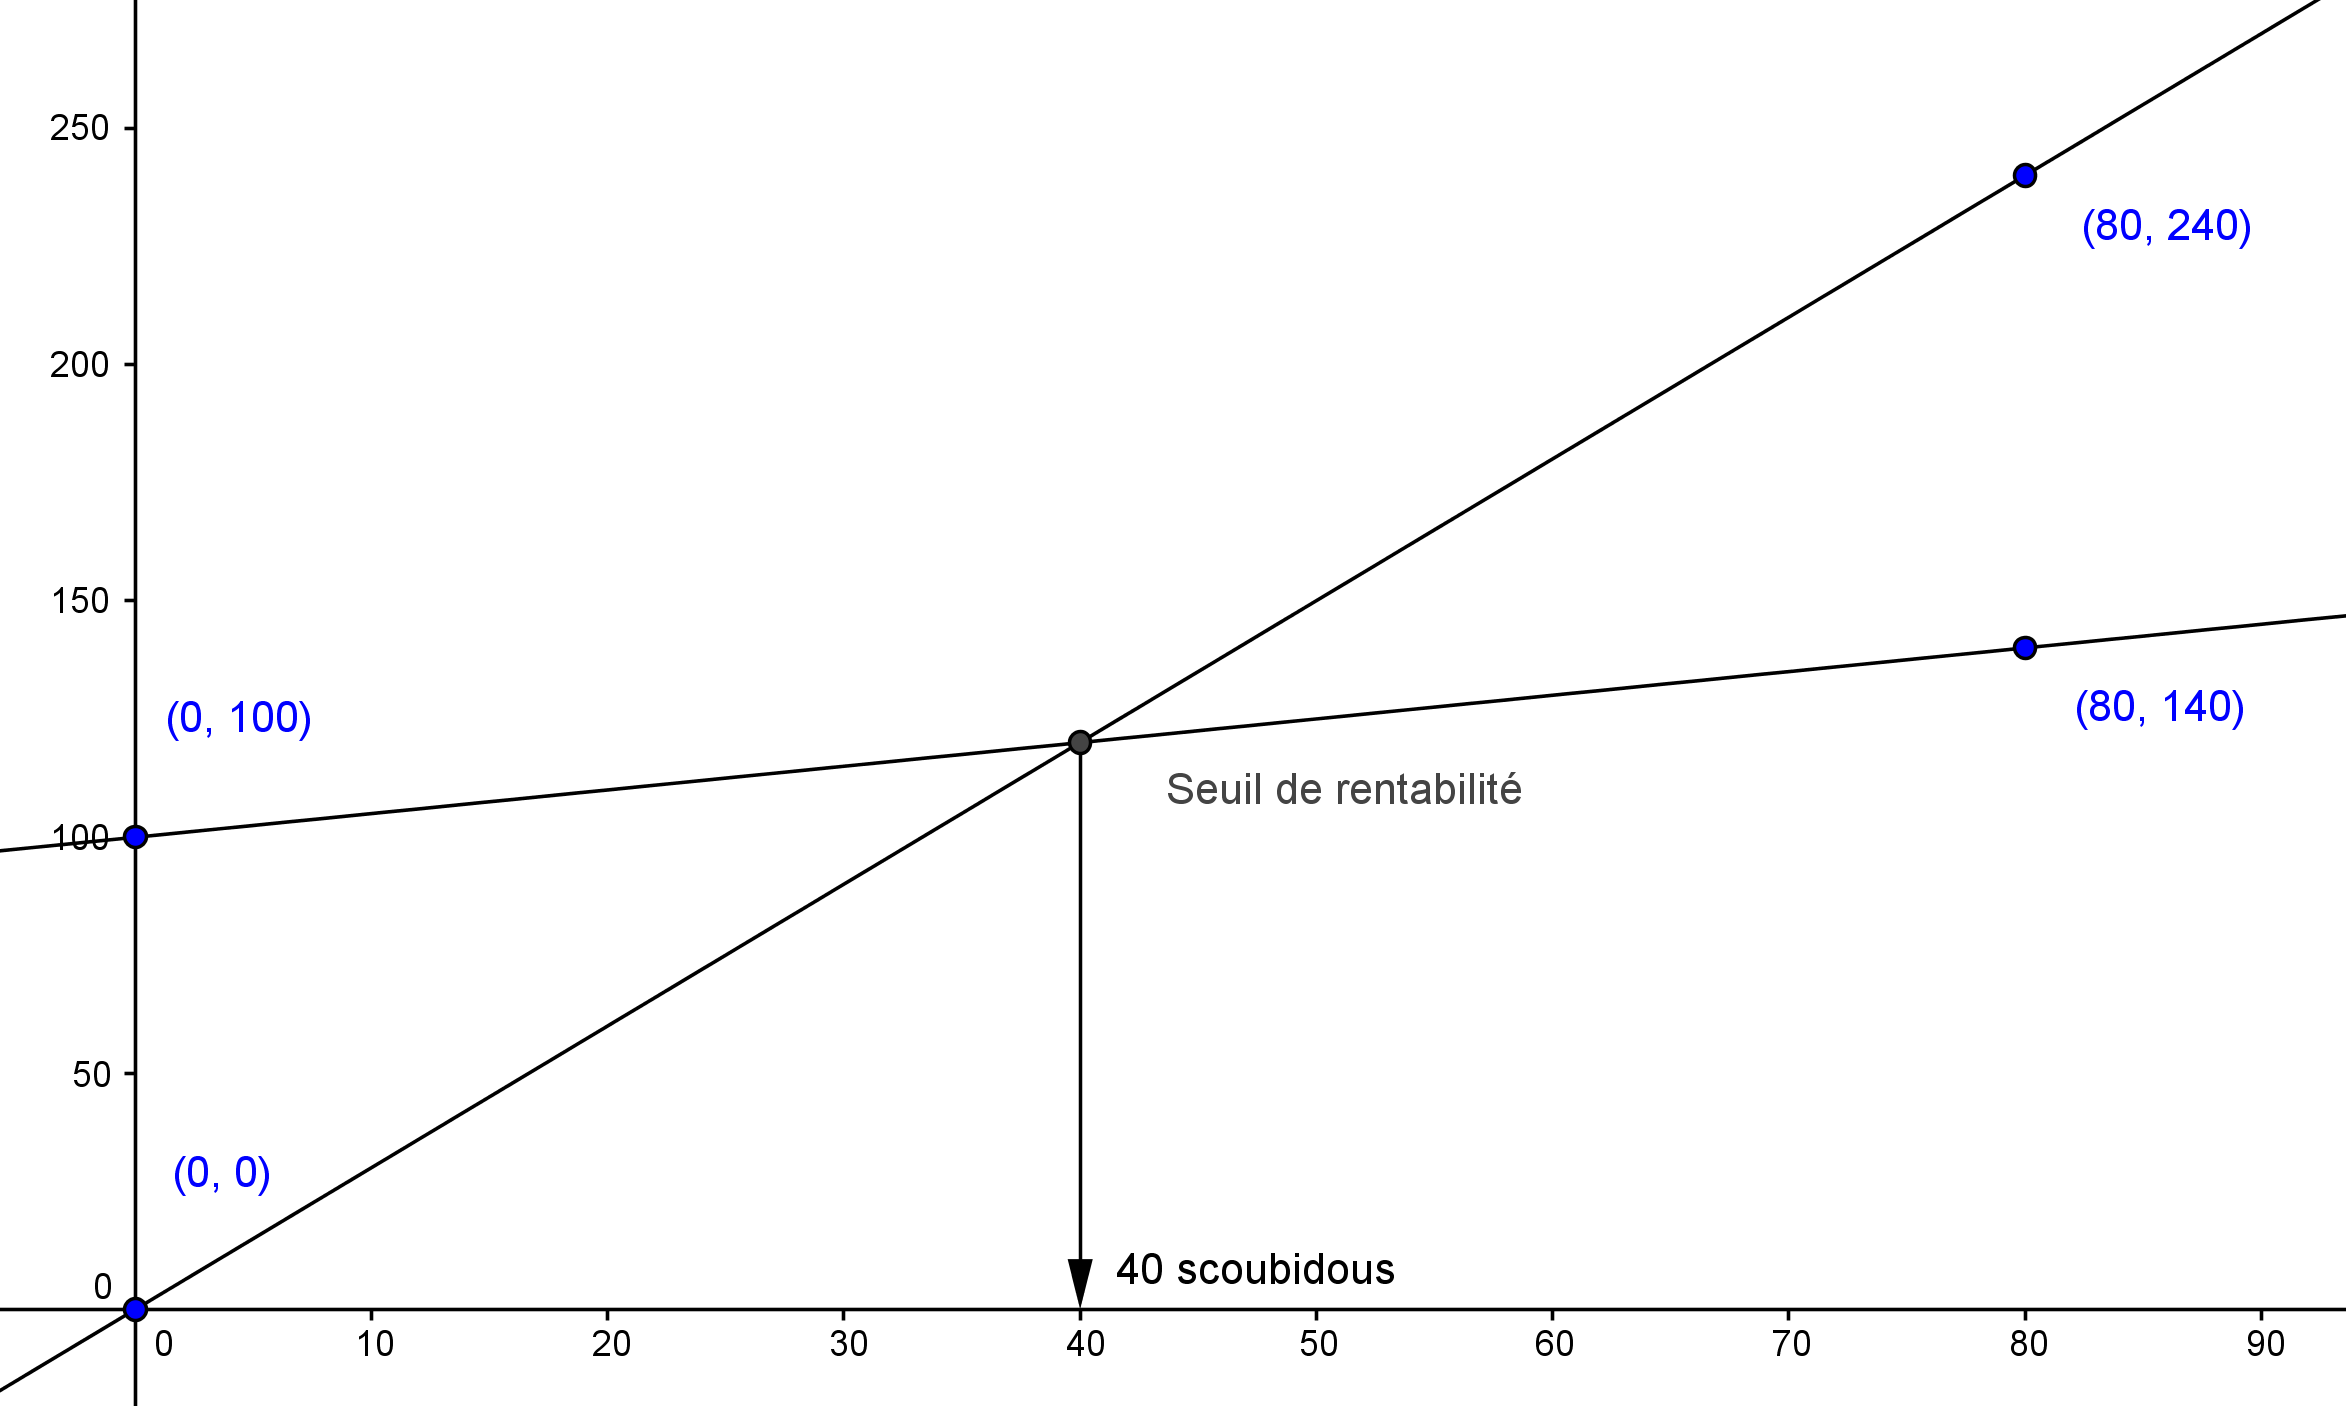
\includegraphics[width=0.7\textwidth]{rentabilite/seuil_ex.png}
\end{center}
Pour faciliter la représentation, il est souvent nécessaire de ne pas utiliser la même graduation pour les deux axes !
\end{exemple}

\section{Comparatif d'offres}

Cette section peut paraître n'avoir aucun lien avec le chapitre, mais le raisonnement est le même que pour les seuils de rentabilité.

On s'intéresse ici à plusieurs offres portant sur la même matière (par exemple : payer tous ses  trajets, prendre un demi-tarif ou un abonnement général) et on cherche à analyser l'offre. Par exemple, à partir de combien de trajets prendre un demi tarif est-il plus avantageux que de payer en plein chaque déplacement ?

Pour cela, nous allons commencer par décrire la fonction liée à chaque offre, représenter son graphe et nous intéresser aux points d'intersection (on commence à voir le rapport avec le seuil de rentabilité).

\begin{exemple}
Jean-Paul fait régulièrement le trajet Martigny-Genève. Il paye son billet $41$ Frs. Le demi-tarif est à $185$ Frs par année et l'abonnement général à $3655$ Frs par année. Que conseiller à Jean-Paul ?

Soit $x$ le nombre de trajets que Jean-Paul effectue par année, $h(x)$ ce qu'il paye avec des billets normaux, $i(x)$ avec le demi-tarif et $j(x)$ avec l'abonnement général. On peut assez vite deviner :
$$
\left\{
\begin{array}{l}
h(x) = 41 x\\
i(x) = \frac{41}{2} x + 185\\
j(x) = 3655
\end{array}
\right.
$$
On fait donc le graphique suivant :
\begin{center}
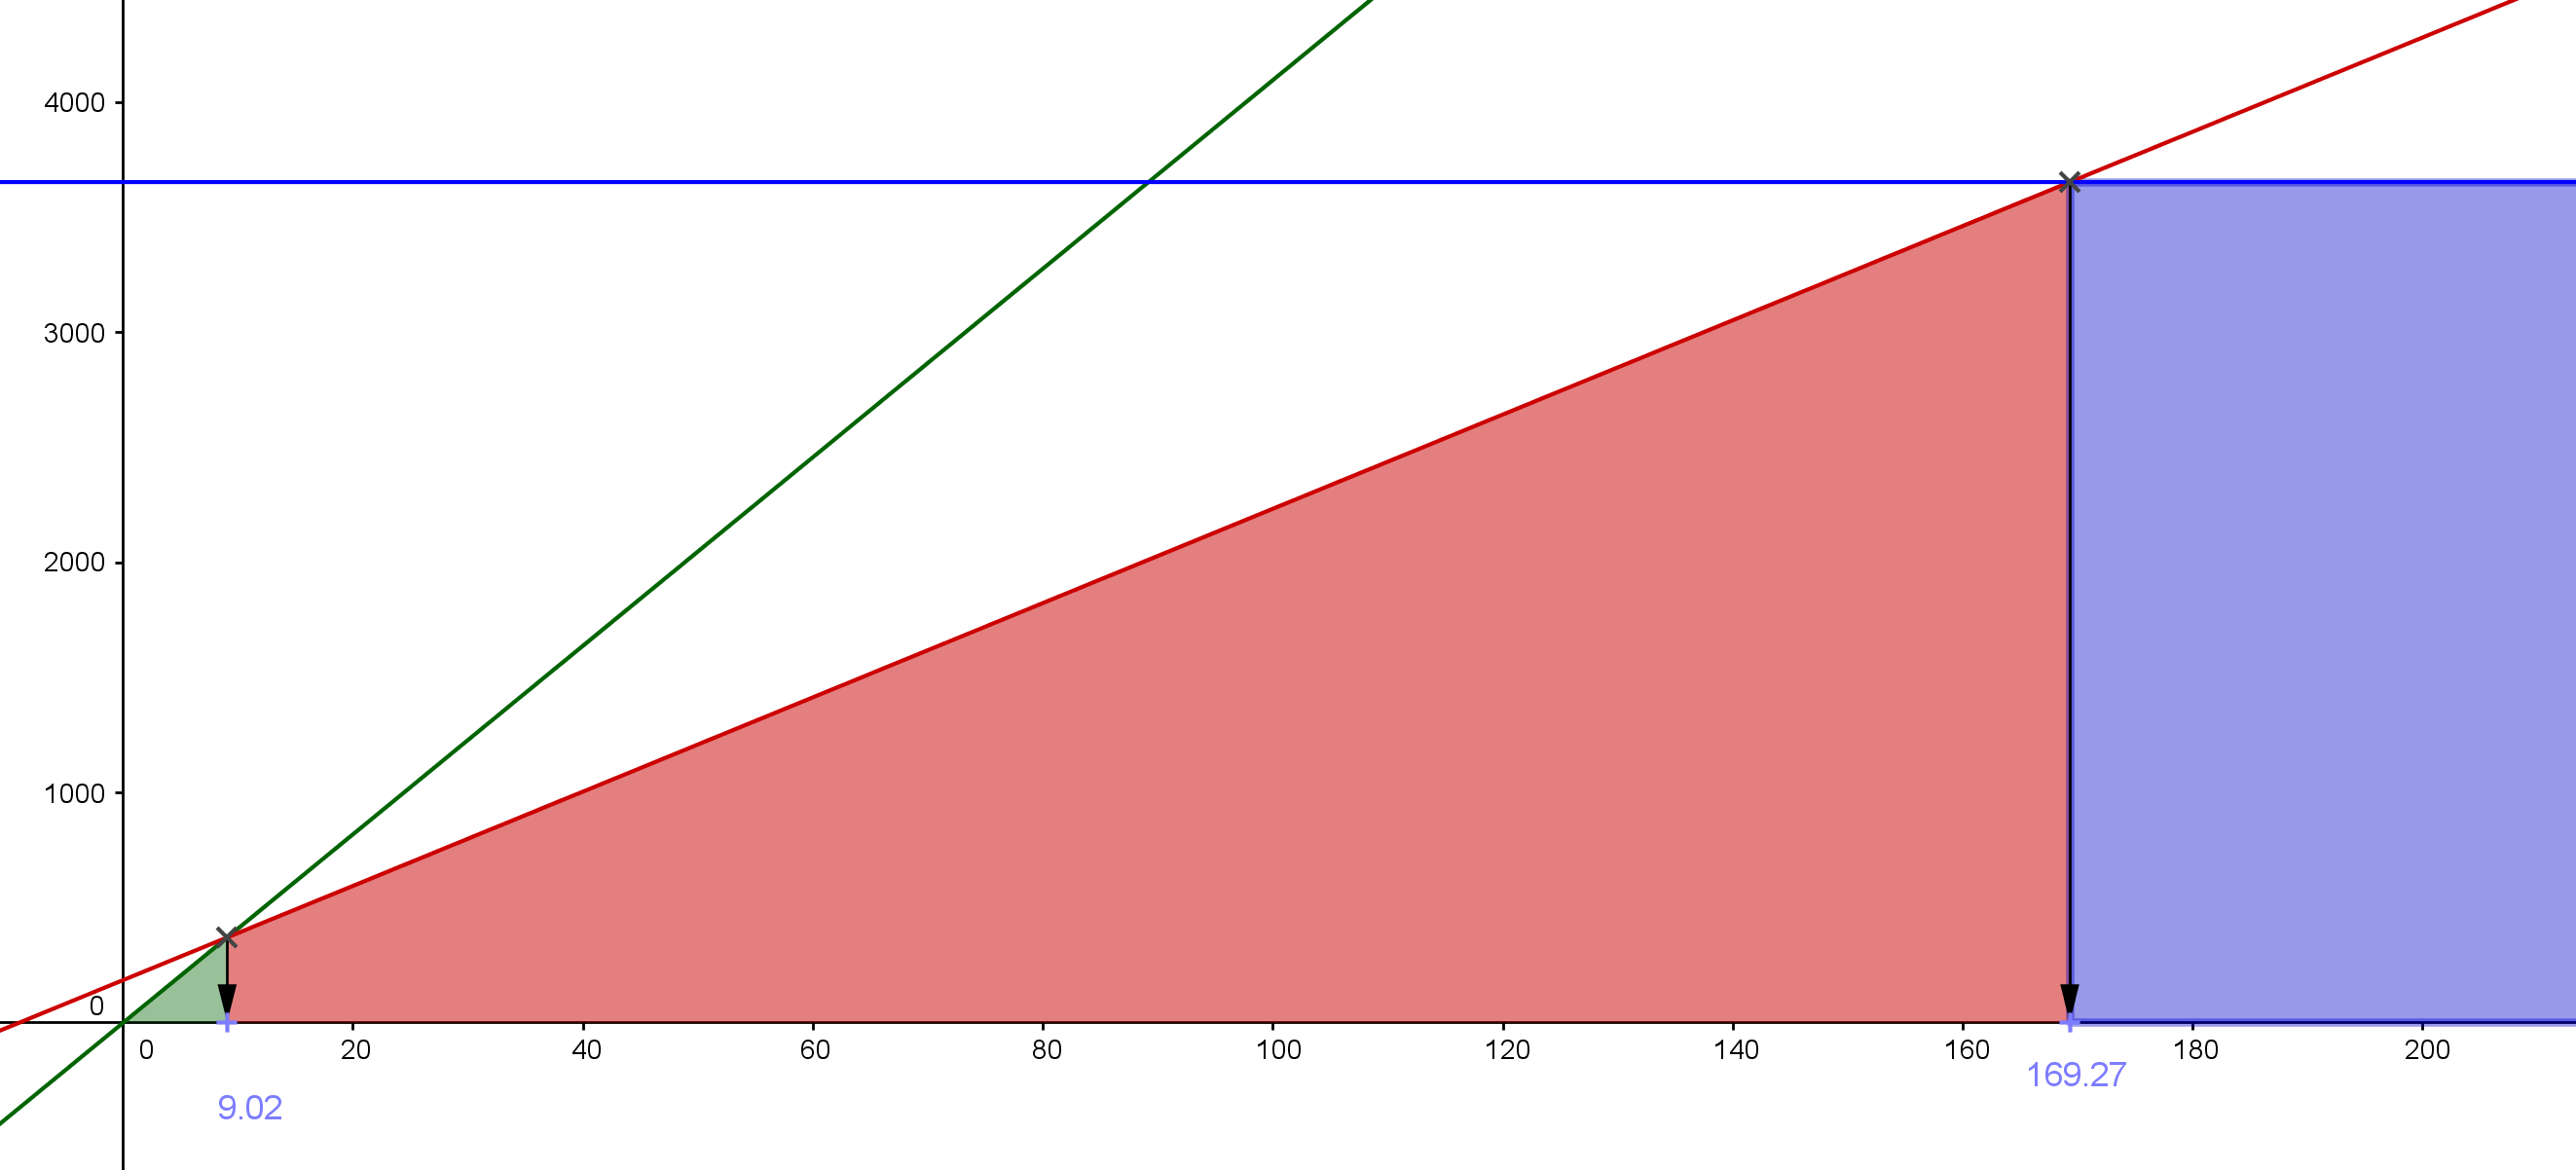
\includegraphics[width = 0.9 \textwidth]{rentabilite/comparatif.png}
\end{center}
Ainsi dans la première zone, la fonction $h$ est la plus avantageuse, la deuxième, la fonction $i$ et la dernière la fonction $j$.

Il nous faut à présent trouver les pivots des zones. On les trouve à l'intersection des fonctions $h$ et $i$ ainsi qu'à celle des fonctions $i$ et $j$. L'intersection des fonctions $h$ et $j$ ne nous intéresse pas, comme on le voit sur le graphique.

Commençons par les fonctions $h$ et $i$ :
$$
\begin{array}{lcl}
41 x &=& \frac{41}{2} x + 185 \ssi \\
41x - \frac{41}{2}x = 185 \ssi \\
\frac{41}{2} x = 185 \ssi \\
x = \frac{370}{41} \simeq 9,02
\end{array}
$$
puis par celle des fonctions $i$ et $j$
$$
\begin{array}{lcl}
\frac{41}{2}x + 185 &=& 3655 \ssi \\
\frac{41}{2} x &=& 3470 \ssi \\
x = \frac{6940}{41} \simeq 169,27
\end{array}
$$
Ainsi si Jean-Paul effectue entre $0$ et $9$ trajets par an, il préférera payer ses trajets en plein, entre $10$ et $169$ trajets, il prendra un demi-tarif, au-delà de $170$ trajets, il prendra un abonnement général.
\end{exemple}

\section{Exercices}

\begin{exercice}
Francine gère un comptoir où elle vend des soupes. Elle a calculé que son coût de production quotidien est constitué de Fr. 42.— de frais fixes plus Fr. 0,60 par soupe qu’elle prépare. Elle vend ses soupes Fr. 1.— chacune. Trouver le nombre de soupes qu’elle doit vendre dans une journée pour atteindre le seuil de rentabilité.
\end{exercice}

\begin{exercice}
Un maraîcher sait qu’il peut vendre toute sa production de navets en les vendant Fr. 0,40 chacun. Il estime qu’il a des frais fixes de Fr. 100.— par jour et qu’il lui en coûte Fr. 0,20 pour produire chaque navet. Trouver son seuil de rentabilité.
Un vendeur de machines agricoles propose à ce maraîcher l’achat d’une machine qui réduira le coût de production à Fr. 0,10 par navet mais qui augmentera ses frais fixes à Fr. 180.— par jour. Analyser le seuil de rentabilité et les coûts de production pour aider le producteur à prendre une décision.
\end{exercice}

\begin{exercice}
Un marchand achète d’un grossiste des bas pour hommes au prix de Fr. 2.— chaque paire. Si les frais fixes de fonctionnement de la mercerie sont de Fr. 148.— par jour, à quel prix devra-t-il vendre chaque paire de bas pour avoir un seuil de rentabilité de 37 paires par jour ?
\end{exercice}

\begin{exercice}
Un éditeur décide de publier un ouvrage de mathématiques. Les coûts qu’il doit assumer sont formés de frais fixes (composition, montage) s’élevant à Fr. 12'240.— et de frais variables (impression, droits d’auteurs) s’élevant à Fr. 9.— par volume. S’il vend ses livres Fr. 21.— chacun, trouver son seuil de rentabilité.
Un nouveau procédé de composition permet de baisser les frais fixes à Fr. 9'660.—. Par contre, dans ce cas, l’impression fait grimper les coûts variables à Fr. 11.— par livre. Analyser le seuil de rentabilité.
\end{exercice}

\begin{exercice}
On désire donner de la fabrication en sous-traitance ; trois entreprises font les propositions suivantes :
A : Fr. 150.— la pièce
B : Fr.   75.— la pièce + un investissement unique de Fr. 1'000.—
C : Fr.   50.— la pièce + un investissement unique de Fr. 2'000.—
Illustrer ces trois propositions par un graphique, calculer les seuils de rentabilité et enfin analyser concrètement les trois propositions.
\end{exercice}

\begin{exercice}
Un propriétaire encaveur produit chaque année 25'000 bouteilles. Il vend Fr. 145.–– les dix bouteilles.
Il paie annuellement les frais fixes suivants : 
amortissement des installations	Fr. 12'100.—
assurances	Fr.   9'500.—
chauffage	Fr.   5'300.––
divers	Fr.   5'200.––
 
 
Ainsi que les frais variables suivants par bouteille : 
bouteille	Fr. 0.45
bouchon	Fr. 0.10
étiquette	Fr. 0.30
acide sulfurique	Fr. 0.05
petit matériel	Fr. 0.55
vin	Fr. 7.05
 

Quel doit être le nombre de bouteilles à vendre pour couvrir ses frais fixes ?
S'il vend les 25'000 bouteilles, quel bénéfice fera-t-il ?
Après deux années d'exploitation, il décide de baisser le prix de vente de 10 %. Quel sera le nouveau seuil de rentabilité ?
Un pépiniériste prépare une plantation de thuyas ; pour cela, il loue un terrain agricole d’un hectare sur lequel il plantera ses jeunes arbustes ; la location annuelle du terrain s’élève à Fr. 0.25 le m2 (1 hectare = 10'000 m2).
\end{exercice}

\begin{exercice}
L’entretien des jeunes arbres (heures de travail, engrais, machines, …) s’élève à Fr. 0.75.–– par arbuste et par année.

Il s’écoule exactement quatre années entre la date de la plantation et la date de la vente des thuyas.

Le prix de vente d’un thuya étant de Fr. 5.––, calculer le nombre de thuyas que devra vendre le pépiniériste pour qu’il puisse rentrer dans ses frais.

Sachant qu’il a planté et cultivé 60'000 thuyas et qu’après 4 ans il ne pourra en vendre que le $90 \%$, calculer le revenu annuel moyen que lui procurera la vente des arbres ?
\end{exercice}

\begin{exercice}
Les CFF proposent 3 possibilités de paiement :

Payer le trajet en plein tarif 
Acheter un abonnement demi-tarif de Fr. 150.— et payer le trajet à moitié prix
Acheter un abonnement général de Fr. 1050.— et ne pas payer le trajet 

Monsieur Blanc prend le train fréquemment en direction de Sion. 
Son trajet aller-retour lui coûte Fr. 12,50 en plein tarif. Il hésite entre payer son billet toutes les semaines ou opter pour un abonnement (demi-tarif ou général). 

Que conseiller à Monsieur Blanc ?

Représenter la situation graphiquement.
\end{exercice}

\section{Corrigés}

\begin{solution}
Seuil de rentabilité $ {  : x}=\frac{42}{1-0.6}=105$

\begin{tikzpicture}
\begin{axis}[
    xmin=0, xmax=150,
    ymin=0, ymax=160,
    axis lines=center,
    axis on top=true,
    domain=0:150,
    nodes near coords,
    point meta=explicit symbolic,
    height=8cm,width=\textwidth,
    ]

   	\addplot [mark=none,draw=red, thick] {0.6*x+42};
	\addplot [mark=none,draw=blue, thick] {x};
	\addplot+[only marks] coordinates{(105,105)[$(105 ;105)$]} ;
\end{axis}
\end{tikzpicture}
\end{solution}

\begin{solution}
Seuil de rentabilité $ {  1 : x}=\frac{100}{0.4-0.2}=500$	
Seuil de rentabilité $ {  2 : x}=\frac{180}{0.4-0.1}=600$

\begin{tikzpicture}
\begin{axis}[
    xmin=0, xmax=1000,
    ymin=0, ymax=450,
    axis lines=center,
    axis on top=true,
    domain=0:1000,
    nodes near coords,
    point meta=explicit symbolic,
    height=8cm,width=\textwidth,
    ]

   	\addplot [mark=none,draw=red, thick] {0.2*x+100};
	\addplot [mark=none,draw=green, thick] {0.1*x+180};
	\addplot [mark=none,draw=blue, thick] {0.4*x};
	\addplot+[only marks] coordinates{(500,200)[$(500 ;200)$]} ;
	\addplot+[only marks] coordinates{(600,240)[$(600 ;240)$]} ;
\end{axis}
\end{tikzpicture}
\end{solution}

\begin{solution}
$37=\frac{148}{x-2}\Leftrightarrow 37x-74=148\Leftrightarrow 37x=222\Leftrightarrow x=6$
\end{solution}

\begin{solution}
Seuil de rentabilité $ {  1 : x}=\frac{12'240}{21-9}=1'020$

Seuil de rentabilité $ {  2 : x}=\frac{9'660}{21-11}=966$


\begin{tikzpicture}
\begin{axis}[
    xmin=0, xmax=1600,
    ymin=0, ymax=35000,
    axis lines=center,
    axis on top=true,
    domain=0:1600,
    nodes near coords,
    point meta=explicit symbolic,
    height=8cm,width=\textwidth,
    ]

   	\addplot [mark=none,draw=red, thick] {9*x+12240};
	\addplot [mark=none,draw=green, thick] {11*x+9660};
	\addplot [mark=none,draw=blue, thick] {21*x};
	\addplot+[only marks] coordinates{(966,20286)[$(966 ;20286)$]} ;
	\addplot+[only marks] coordinates{(1020,21420)[$(1020 ;21420)$]} ;
	\addplot+[only marks] coordinates{(1290,23850)[$(1290 ;23850)$]} ;
\end{axis}
\end{tikzpicture}
\end{solution}

\begin{solution}
Seuil de rentabilité $ {  1 : x}=\frac{1000}{150-75}\cong 14$	

Seuil de rentabilité $ {  2 : x}=\frac{2000-1000}{75-50}=40$
 De 0 à 13 : proposition A	De 14 à 40 : proposition B	A partir de 41 : proposition C


\begin{tikzpicture}
\begin{axis}[
    xmin=0, xmax=50,
    ymin=0, ymax=8000,
    axis lines=center,
    axis on top=true,
    domain=0:50,
    nodes near coords,
    point meta=explicit symbolic,
    height=8cm,width=\textwidth,
    ]

   	\addplot [mark=none,draw=red, thick] {75*x+1000};
	\addplot [mark=none,draw=green, thick] {50*x+2000};
	\addplot [mark=none,draw=blue, thick] {150*x};
	\addplot+[only marks] coordinates{(13.3,2000)[$(13.3 ;2000)$]} ;
	\addplot+[only marks] coordinates{(40,4000)[$(40 ;4000)$]} ;
\end{axis}
\end{tikzpicture}
\end{solution}

\begin{solution}
Frais fixes : Fr. 32'100.—, frais variables : Fr. 8.5

Seuil de rentabilité $ {  1 : x}=\frac{32'100}{14.5-8.5}=5'350$

Bénéfice :\[\]$25'000\cdot \left( 14.5-8.5 \right)-32'100=117'900$ 

Nouveau prix de vente : Fr. 13.05, Seuil de rentabilité $ {  2 : x}=\frac{32'100}{13.05-8.5}\cong 7'055$

\begin{tikzpicture}
\begin{axis}[
    xmin=0, xmax=7500,
    ymin=0, ymax=140000,
    axis lines=center,
    axis on top=true,
    domain=0:7500,
    nodes near coords,
    point meta=explicit symbolic,
    height=8cm,width=\textwidth,
    ]

   	\addplot [mark=none,draw=red, thick] {8.5*x+32100};
	\addplot [mark=none,draw=green, thick] {14.5*x};
	\addplot [mark=none,draw=blue, thick] {13.05*x};
	\addplot+[only marks] coordinates{(5350,77575)[$(5350 ;77575)$]} ;
	\addplot+[only marks] coordinates{(7055,92068)[$(7055 ;92068)$]} ;
\end{axis}
\end{tikzpicture}
\end{solution}

\begin{solution}
Prix de la location pour 4 ans : Fr. 10'000.—, Entretien d’un arbre pour 4 ans : Fr. 3.—

Seuil de rentabilité $ {   : x}=\frac{10'000}{5-3}=5'000$

Revenu  annuel : $\frac{54'000\cdot 5-60'000\cdot 3-10'000}{4}=Fr.\text{ }20'000$

\begin{tikzpicture}
\begin{axis}[
    xmin=0, xmax=6000,
    ymin=0, ymax=35000,
    axis lines=center,
    axis on top=true,
    domain=0:6000,
    nodes near coords,
    point meta=explicit symbolic,
    height=8cm,width=\textwidth,
    ]

   	\addplot [mark=none,draw=red, thick] {5*x};
	\addplot [mark=none,draw=green, thick] {3*x+10000};
	\addplot+[only marks] coordinates{(5000,25000)[$(5000 ;25000)$]} ;
\end{axis}
\end{tikzpicture}
\end{solution}

\begin{solution}
Seuil de rentabilité $ {  1 : x}=\frac{150}{12.5-6.25}=24$

Seuil de rentabilité $ {  2 : x}=\frac{1'050-150}{6.25}=144$

\begin{tikzpicture}
\begin{axis}[
    xmin=0, xmax=150,
    ymin=0, ymax=1200,
    axis lines=center,
    axis on top=true,
    domain=0:150,
    nodes near coords,
    point meta=explicit symbolic,
    height=8cm,width=\textwidth,
    ]

   	\addplot [mark=none,draw=red, thick] {12.5*x};
	\addplot [mark=none,draw=green, thick] {6.25*x+150};
	\addplot [mark=none,draw=blue, thick] {1050};
	\addplot+[only marks] coordinates{(24,300)[$(24 ;300)$]} ;
	\addplot+[only marks] coordinates{(144,1050)[$(144 ;1050)$]} ;
\end{axis}
\end{tikzpicture}
\end{solution}



